\maketitle
\section*{The Universe}
In the beginning the Universe was created. This has made a lot of people very angry and been widely regarded as a bad move.
I know what I did to make so many people so angry, but it really just sounds like their problem.

In figure \ref{fig:universe} you can see a picture of a galaxy.

\begin{figure}[h]
  \center
  \includegraphics[width=0.6\textwidth]{galaxy.jpg}
  \caption{A picture of a galaxy}
  \label{fig:universe}
\end{figure}

A galaxy is really big. You're just a tiny spec of dust in comparison. Now, there are a lot of galaxies in the universe.
So many indeed, that there are galaxy clusters, where multiple galaxies are grouped together based on the distance between them.
But that's not enough yet. There are also clusters of clusters. And then there's groups of clusters.

The universe is really big. We don't even really know how big. Why? We can't even see it's borders, because light from there hasn't reached us yet.

In a believed stroke of genius, some may say that there's still something more massive, your mom. However, since we're here to proof that you're insignificant,
your mom can't be this massive, or it would be something you'd be significant for.

\pagebreak

\section{The Beginning}

Now let's talk about how everything came to be. Since, you know, I'm God, I have utmost authority when speaking about the beginning of times.

Now, in another believed stroke of genius, some may say that everything came to be, because I fucked your mom. However, I'm God, so I have higher standards.

What actually happened, is that I just felt like torturing some innocent souls of the aether for existing, so I just made an endless place of torment to place them into.
This has backfired immensly though, because somehow, somewhy, some people believe that there's a way to salvation and that I love them and so on. I don't really know how the fuck
you'd think that, but you do you. Now I could end this paper here and have you conclude on your own that you're insignificant, because I obviously created you to torture you, but
I feel like shitting on you some more, so this is only \emph{the Beginning}.

\begin{center}
  Have fun!
\end{center}
\section{Your Beginning}

It doesn't matter.
\section{Your Life}

Holy fuck, how did you even get this far? Your life has no meaning, you have no reason to exist. Why didn't you kill yourself already?
Well, since you're here anyways, I can prove to you how you existing does not add anything to the universe at all.
Let $a : \text{Person} \rightarrow \mathbb{N}$, with 
$$a(x) = \text{number of meaningful achievemnts of } x$$
where $x \in \text{Person}$.

Now you might think that on a bell curve of intelligence, like the one shown in 
figure \ref{fig:bell-curve}, the graph plotting the average of 
$$a(x_1), a(x_2), \dotsc, a(x_{n-1}), a(x_n)$$
with $x_i \in \{x \in \text{Person } | \text{ IQ of } x \text{ is the current IQ}\}$ over the IQ, would resemble an exponential one, because
you'd think that the more intelligent someone was, the more they would achieve in their life. I would wager that the vast amount of people
think like this. However, it isn't true.

\begin{figure}[h]
  \center
  \includegraphics[width=0.8\textwidth]{bell-curve.jpg}
  \caption{The intelligence bell curve}
  \label{fig:bell-curve}
\end{figure}

Another thing you might think is that it could also behave like the bell curve itself. The reasoning behind it might be the conclusion that
once you become too intelligent, you overthink a lot and it prevents you from actually getting things done.

\pagebreak

However, I'm here to tell you that it would probably rather look something like the graph shown in figure \ref{fig:graph-achievements}.
Why do I say that? Well, because no human being has ever achieved something meaningful. Nothing you or anybody else has ever done has
contributed something to the universe. And I'm certain of that, because I made it that way.

\begin{figure}[h]
  \center
  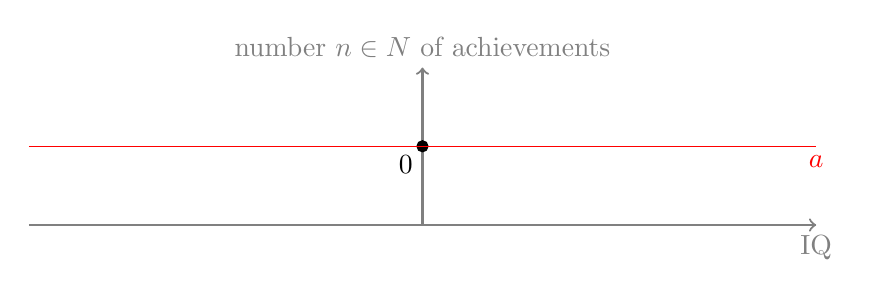
\begin{tikzpicture}
    \draw[->, gray, thick] (-5, -1) -- (5, -1) node[anchor=north]{IQ};
    \draw[->, gray, thick] (0, -1) -- (0, 1) node[anchor=south]{number $n \in \mathbb{N}$ of achievements};
    \filldraw[black] (0,0) circle (2pt) node[anchor=north east]{0};
    \draw[red, thin] (-5, 0) -- (5, 0) node[anchor=north]{$a$};
  \end{tikzpicture}
  \caption{Average amount of meaningful achievements per step of IQ}
  \label{fig:graph-achievements}
\end{figure}